\chapter{Регрессионное тестирование}

Регрессионное тестирование — это выборочное тестирование, позволяющее
убедиться, что изменения не вызвали нежелательных побочных эффектов, или что
измененная система по-прежнему соответствует требованиям.
Для того чтобы знать, какие тесты перезапускать после того или иного изменения в
программе, нужно определить, от каких конкретно частей программы (модулей, методов,
и т.п.) зависит результат каждого теста. Для этого часто используется управляющий
граф , отображающий поток управления программы, по которому легко отследить
зависимости одних блоков/модулей/методов от других.

Был построен один из вариантов управляющего графа: граф вызовов ,
показывающий, какие методы или функции вызывают какие. Граф был построен с
помощью утилиты NDepend. Так как я хотел провести регрессионное вместе с автоматизированным, то было решено протестировать те части кода, которые не зависят от базы данных и могут быть выполнены на стороне удаленной виртуальной машины. Поэтому для регрессионного и автоматизированного тестирования были выбраны Mock-тесты. 
 
\begin{table}
\caption{\label{tab:block_graph-test} Матрица вызовов Mock-тестов}
\begin{center}
\begin{tabular}{|l|c|c|c|c|}

\hline
 & \multicolumn{4}{|c|}{Методы} \\
\hline
Тесты & SelectAllUsers() & InsertUser() & FindUser() & DeleteGroup()\\
\hline
GetAllUsersTest & + & - & - & -\\
\hline
InsertUserTest & - & + & - & -\\
\hline
FindUserTest & - & - & + & -\\
\hline
TestDeletion & - & - & - & +\\
\hline
UpdateUserTest& + & - & - & -\\
\hline

\end{tabular}
\end{center}
\end{table} 

\begin{figure}
	\centering
	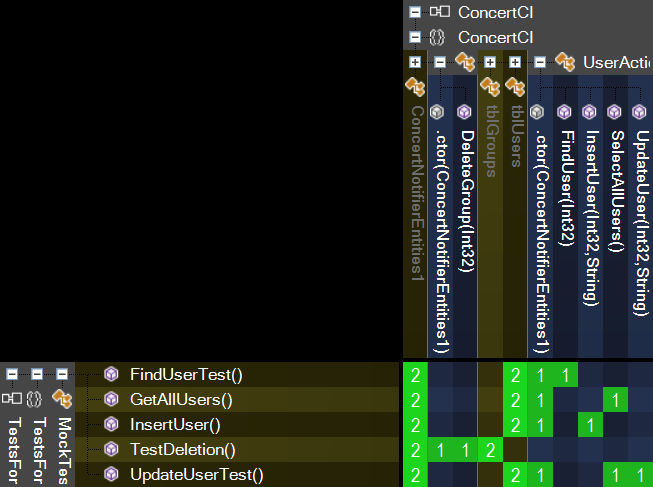
\includegraphics[scale=0.7]{DependencyMatrixSmall.png}
	\caption{Матрица вызовов для Mock-тестов, построенная NDepend}
	\label{image:simple-dep}
\end{figure}


\begin{figure}
	\centering
	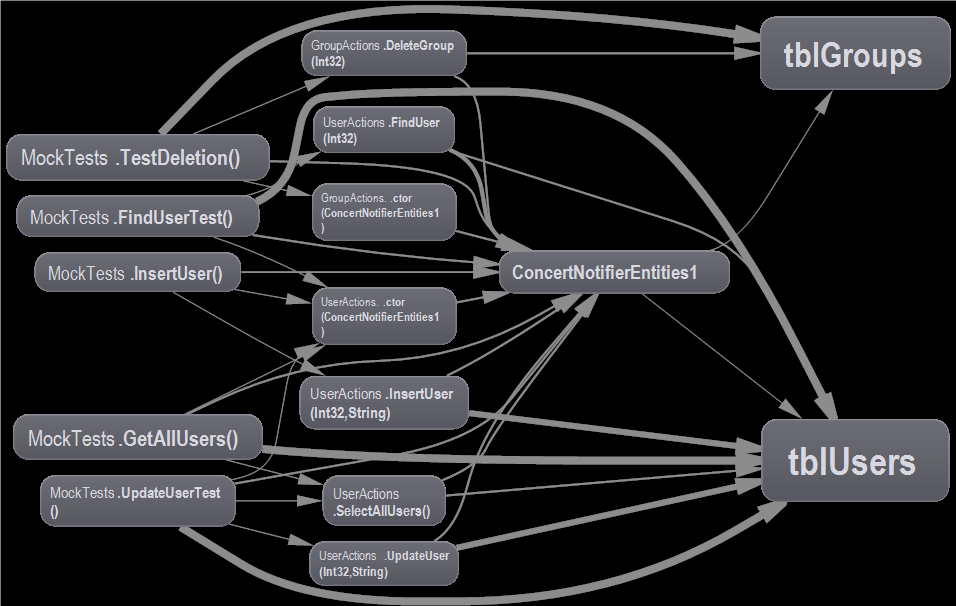
\includegraphics[scale=0.7]{DependencyGraphSnapshotSimple.png}
	\caption{Граф вызовов для Mock-тестов, построенный NDepend} 
	\label{image:simple-graph}
\end{figure}

\newpage
В данном сценарии Mock-тестов мы изменили все методы, добавив обработку исключений с помощью оператора try-catch. Все тесты были успешно пройдены после добавления обработки исключений, поэтому было решено намерено допустить ошибку в методе DeleteGroup(), чтобы проверить случай, при котором не все тесты удачно пройдут автоматизированное тестирование. Подробнее это описано в следующем разделе под названием \textbf{ "Автоматизированное тестирование"}

Было решено также построить матрицу вызовов для всех тестов, используя NDepend. 
Граф вызовов из-за высокого разрешения не был приложен к отчету, но может быть найден в папке с отчетом как и все остальные иллюстрации данного отчета.
\begin{figure}
	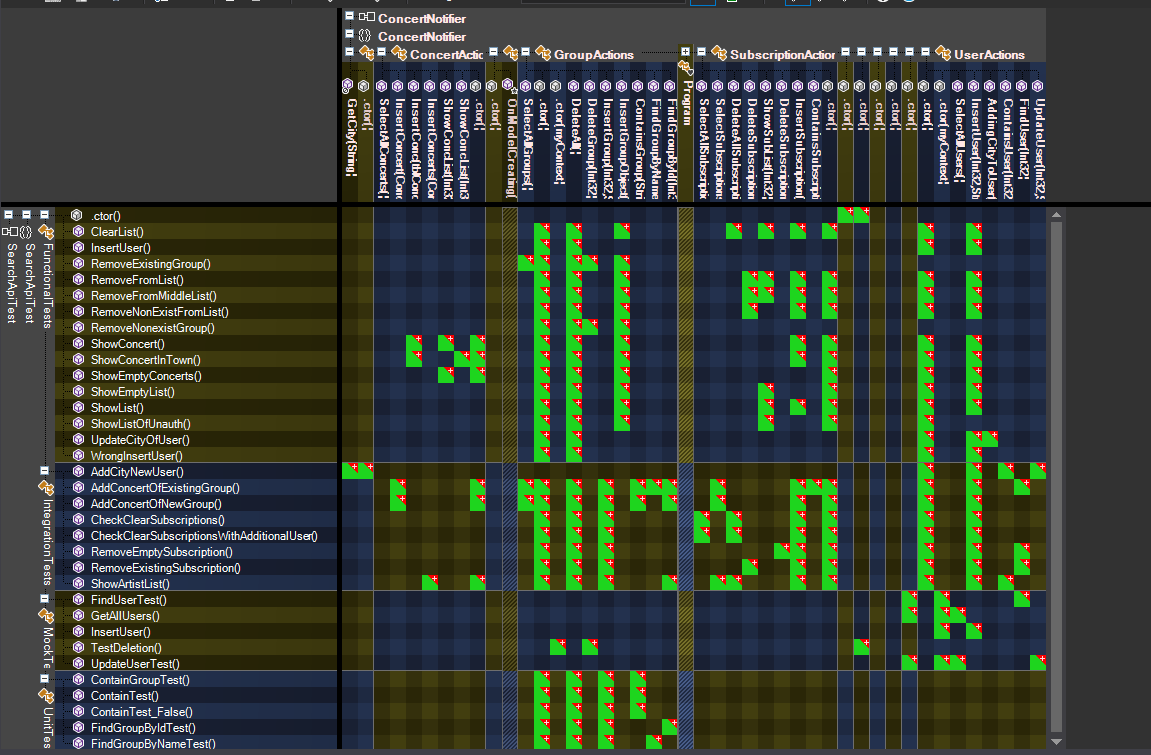
\includegraphics[scale=0.63]{MatrixDep.PNG}
	\caption{Прохождение тестов до изменения блока K}
	\label{image:complex-dep}
\end{figure}



\chapter{Автоматизированное тестирование}
Реализация тестов — достаточно затратный процесс, поэтому часто прибегают к тем
или иным средствам, его облегчающим. В данной лабораторной работе для автоматизированного тестирования использовался ресурс \textbf{Travis CI}. Данный ресурс позволяет проверять работоспособность проекта, после каждого обновления репозитория на GitHub, запуская проект на удаленной виртуальной машине и выводя результаты в виде мини-отчета. 
Для этого проект с Mock-тестами был загружен на ресурс GitHub и к нему был подключен Travis CI и написан скрипт для сборки проекта.

\begin{lstlisting}[caption={Сценарий сборки для Travis CI}, label={lst:set-info}]
language: csharp
solution: ConcertCI.sln
before_install:
- sudo apt-get install nunit-console
before_script:
- nuget restore ConcertCI.sln
after_script:
- nunit-console TestsForCI/bin/Release/TestsForCI.dll 
\end{lstlisting}

После этого был рассмотрен случай изменения метода DeleteGroup(), который был разобран в предыдущем разделе.
\begin{figure}
	\centering
	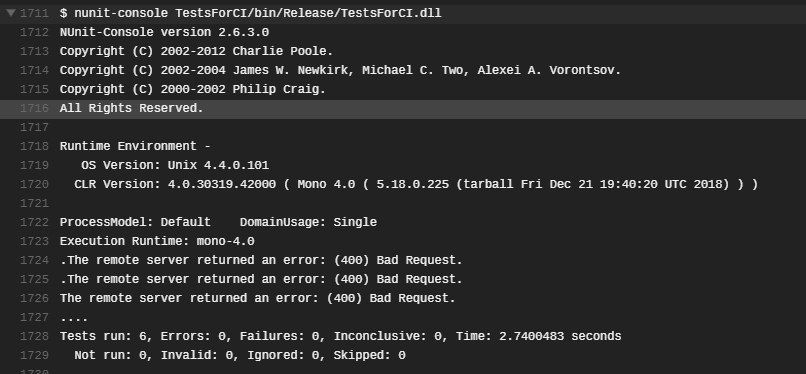
\includegraphics[scale=1]{Before.PNG}
	\caption{Прохождение тестов до изменения метода DeleteGroup()}
	\label{image:beforedelete-edit}
\end{figure}

\begin{figure}
	\centering
	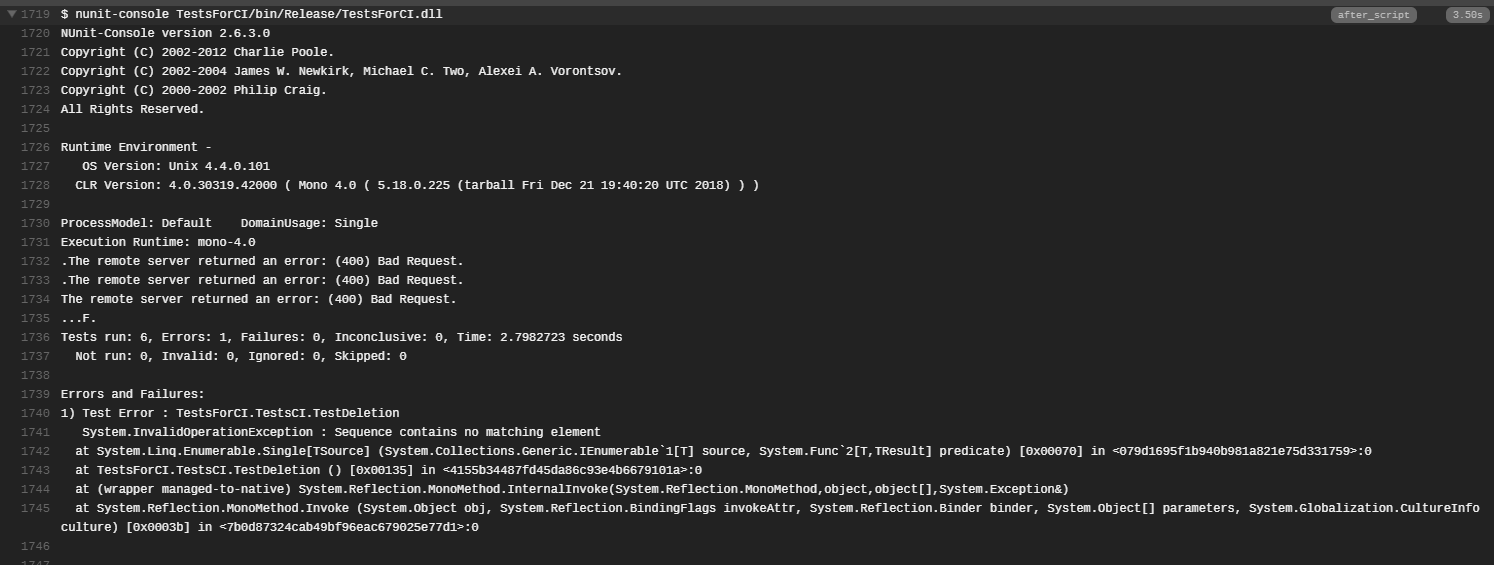
\includegraphics[scale=1]{After.PNG}
	\caption{Прохождение тестов после изменения метода DeleteGroup()}
	\label{image:afterdelete-edit}
\end{figure}

